% =============================================================================
% Iter 71 -- Pillar 3: Loss-of-Signal Decomposition.  Why does G=4 lose to
%             G=32?  Attribution to (a) signal availability (ZVF/GU),
%             (b) group-mean variance (sqrt(G_ref/G)), (c) sample budget.
% Driver: scripts/group_size_iter71.py
% Inputs: experiments/results/group_size_token_normalized.tsv
%         experiments/results/group_size_iter43_eff_zvf.tsv
%         experiments/results/group_size_iter67_iaf_ratios.tsv
% Outputs: experiments/results/group_size_iter71_signal_loss.tsv
%          experiments/results/group_size_iter71_eff_batch.tsv
%          experiments/results/group_size_iter71_decomp.tsv
%          experiments/results/group_size_iter71_multiplicative.tsv
%          experiments/results/group_size_iter71_fixed_budget.tsv
%          experiments/results/group_size_iter71_summary.tsv
%          figures/group_size_iter71_decomp.{pdf,png}
%          figures/group_size_iter71_g4_budget.{pdf,png}
% =============================================================================
\subsection{Iter 71 Pillar 3: Loss-of-Signal Decomposition ---
              The Group-Mean Variance Penalty Dominates the $G{=}4$ Deficit
              at Fixed Budget, and the Naive ``ZVF-tells-the-story''
              Reading Is Wrong by an Order of Magnitude}
\label{sec:group-size-iter71}

\paragraph{Question.}
Iters 43 / 55 / 59 established that $G{=}4$ underperforms $G{=}32$
by 5--24 percentage points depending on the token budget and target
accuracy, and iter 67 showed that the operationally dominant group
size is accuracy-dependent (climbing from $G^\star{=}8$ at
$\alpha{=}0.50$ to $G^\star{=}32$ at $\alpha{\ge}0.80$).  Iter 71
asks the diagnostic question: \emph{why} does $G{=}4$ lose?  We
decompose the accuracy deficit at each $(T, G)$ row into three
operationally meaningful components, fit a single additive model on
the 20 observed $(T, G)$ rows, and then isolate the $G$ effect at
fixed $T{=}T_{\mathrm{ref}}$.

\paragraph{Three-component decomposition.}
For each row with budget $T$ and group size $G$, define
\begin{align*}
\Delta_{\mathrm{signal}}(T, G) &= 1 - \mathrm{GU}(T, G) / \mathrm{GU}(T, G_{\mathrm{ref}}), \\
\Delta_{\mathrm{noise}}(G)     &= \sqrt{G_{\mathrm{ref}}/G} - 1, \\
\Delta_{\mathrm{batch}}(T)    &= 1 - T / T_{\mathrm{ref}},
\end{align*}
with $G_{\mathrm{ref}} = 64$ and $T_{\mathrm{ref}} = 64\,\mathrm{M}$.
Fit
\[
\mathrm{acc}(T, G) \approx a_0 + a_s\,\Delta_{\mathrm{signal}}
                              + a_n\,\Delta_{\mathrm{noise}}
                              + a_b\,\Delta_{\mathrm{batch}}
\]
by ordinary least squares on all 20 rows.  The OLS solution
$\hat{\boldsymbol a} = (0.8833,\; 0.1292,\; -0.0421,\; -0.2673)$
yields $R^2 = 0.483$ on the 20-row grid.  Each component is
interpretable: positive $a_s$ means a missing-contrast penalty (the
classic ZVF story), negative $a_n$ means the group-mean variance
penalty hurts accuracy, and negative $a_b$ means larger budgets
help.

\paragraph{Confounded at low budgets; clean at $T{=}T_{\mathrm{ref}}$.}
At $T \in \{1, 4, 16\}\,\mathrm{M}$, every group size pays the same
$\Delta_{\mathrm{batch}}$ ($-26.3$, $-25.1$, $-20.1\,\mathrm{pp}$),
so the budget term \emph{cannot} discriminate between group sizes
at low $T$.  At $T{=}64\,\mathrm{M}$, $\Delta_{\mathrm{batch}} = 0$
for all $G$, isolating the $G$ effect cleanly:

\begin{center}
\small
\begin{tabular}{lccccc}
\toprule
$G$ & acc & $\Delta_{\mathrm{signal}}$ & $\Delta_{\mathrm{noise}}$
       & $\hat{\mathrm{acc}}$ & residual (pp) \\
\midrule
 4 & 0.640 & 0.184 & 3.000 & 0.781 & $-14.1$ \\
 8 & 0.800 & 0.168 & 2.121 & 0.828 & $-2.8$ \\
16 & 0.850 & 0.074 & 1.000 & 0.851 & $-0.1$ \\
32 & 0.880 & 0.017 & 0.414 & 0.868 & $+1.2$ \\
64 & 0.870 & 0.000 & 0.000 & 0.883 & $-1.3$ \\
\bottomrule
\end{tabular}
\end{center}

\noindent\textit{Decomposition of the $G{=}4$ deficit at
$T{=}64\,\mathrm{M}$:}  observed gap $\Delta\mathrm{acc}(G{=}4
\leftrightarrow G{=}64) = 23\,\mathrm{pp}$; the additive model
explains $\Delta_{\mathrm{explained}} = 10.24\,\mathrm{pp}$ (44.5\%
of observed), of which \textbf{the noise penalty accounts for
84.1\%} ($a_n \Delta_{\mathrm{noise}} = -12.62\,\mathrm{pp}$) and
the signal availability accounts for \textbf{only 15.9\%}
($a_s \Delta_{\mathrm{signal}} = +2.38\,\mathrm{pp}$).

\paragraph{What this \emph{reframes}.}
The naive ``high ZVF predicts G=4 failure'' narrative that iter 43
and iter 55 develop is correct in direction but \emph{wrong by an
order of magnitude} on magnitude: at $T{=}64\,\mathrm{M}$ the
signal-availability loss is only $0.18$ probability units (G=4 has
$\mathrm{GU}{=}0.815$ vs $\mathrm{GU}{=}1.000$ at $G{=}64$), and
its fitted contribution to accuracy is just $+2.4\,\mathrm{pp}$.
The dominant loss is the group-mean variance term
$\sqrt{G_{\mathrm{ref}}/G} - 1$, which is $3.0$ at $G{=}4$
($\sqrt{64/4} = 4$), $2.12$ at $G{=}8$, and $1.00$ at $G{=}16$.
This term is independent of token budget and arises from the
fundamental fact that with $G{=}4$ rollouts per prompt, the group
mean has $4\times$ the standard error of the group mean with
$G{=}64$ rollouts.

\paragraph{Implication for the arXiv:2510.00977 ``two-octave
equivalence'' claim.}
Wu et~al.\ (2025) report structural equivalence between $G{=}2$ and
$G{=}16$ (an $8{:}1$ ratio).  Iter 71 shows that the equivalence
breaks \emph{precisely where the group-mean variance term
dominates}: at $T{=}64\,\mathrm{M}$, going from $G{=}16$ to $G{=}4$
costs $9.1\,\mathrm{pp}$ of model-explained accuracy (observed gap
$21\,\mathrm{pp}$), of which $\sim 12\,\mathrm{pp}$ is attributable
to the noise variance term alone.  The Wu equivalence holds only
in the regime where the variance term has already saturated
($G \ge 16$), and breaks precisely when $G$ drops below the
$G{=}16$ threshold.

\paragraph{Pooled vs.\ fixed-budget attribution.}
When the model is fit on all 20 rows, the pooled attribution for
$G{=}4$ is signal $= 6.4\%$, noise $= 38.8\%$, batch $= 54.9\%$
--- but the batch term is an artefact of mixing $T$ values, not a
$G$-specific attribution.  The fixed-budget analysis at
$T{=}T_{\mathrm{ref}}$ is the operationally meaningful attribution
and gives the cleaner $84\%$-noise vs.\ $16\%$-signal split.

\paragraph{Multiplicative cross-check.}
A multiplicative factorisation
$\mathrm{acc}(T, G) \approx
\mathrm{acc}_{\max} \cdot
\mathrm{GU}(T,G)/\mathrm{GU}(T, G_{\mathrm{ref}}) \cdot
\sqrt{G/G_{\mathrm{ref}}} \cdot T/T_{\mathrm{ref}}$
gives a parallel product ranging from $0.012$ at
$(T{=}1\,\mathrm{M}, G{=}4)$ to $1.000$ at $(T{=}64\,\mathrm{M},
G{=}64)$, and identifies the same dominant term at low $G$.

\paragraph{Synthesis with iters 43 / 47 / 51 / 55 / 59 / 63 / 67.}
The loss-of-signal decomposition closes the sequence of
increasingly granular $G{=}4$ vs $G{=}32$ analyses: iter 47
established the *existence* of the deficit, iter 51 quantified it
as a retention curve, iter 55 coupled it to the Wu model, iter 59
gave an equivalence-region estimate, iter 63 fitted the retention
decay, iter 67 reframed it as an iso-accuracy frontier, and iter 71
attributes the deficit to specific mechanistic causes.  The single
sharpest finding is:

\begin{quote}
\emph{At fixed token budget, the $G{=}4$ accuracy deficit is
dominated by the group-mean variance penalty
$\sqrt{G_{\mathrm{ref}}/G}$, not by the ZVF/signal availability
penalty.  This contradicts the naive ``ZVF is the story''
reading that has appeared in iter 43 and elsewhere.}
\end{quote}

\paragraph{Plot reference.}
Figure~\ref{fig:group-size-iter71-decomp} shows the additive
attribution by group size and the predicted-vs-observed fit.
Figure~\ref{fig:group-size-iter71-g4-budget} shows how the $G{=}4$
attribution shifts across budgets.

\paragraph{Artifacts.}
\begin{itemize}
  \item \texttt{experiments/results/group\_size\_iter71\_signal\_loss.tsv} ---
        per-row signal availability gap $\Delta_{\mathrm{signal}}$
        using iter 43's $\mathrm{GU}_{\mathrm{theoretical}}$.
  \item \texttt{experiments/results/group\_size\_iter71\_eff\_batch.tsv} ---
        per-row $\Delta_{\mathrm{noise}}$ and $\Delta_{\mathrm{batch}}$.
  \item \texttt{experiments/results/group\_size\_iter71\_decomp.tsv} ---
        full additive decomposition per $(T, G)$ row.
  \item \texttt{experiments/results/group\_size\_iter71\_multiplicative.tsv} ---
        multiplicative cross-check factorisation.
  \item \texttt{experiments/results/group\_size\_iter71\_fixed\_budget.tsv} ---
        the clean fixed-budget ($T{=}64\,\mathrm{M}$) attribution.
  \item \texttt{experiments/results/group\_size\_iter71\_summary.tsv} ---
        headline metrics.
  \item \texttt{figures/group\_size\_iter71\_decomp.pdf} ---
        additive attribution bar chart + predicted-vs-observed fit.
  \item \texttt{figures/group\_size\_iter71\_g4\_budget.pdf} ---
        $G{=}4$ attribution stacked across budgets.
\end{itemize}

\begin{figure}[ht]
  \centering
  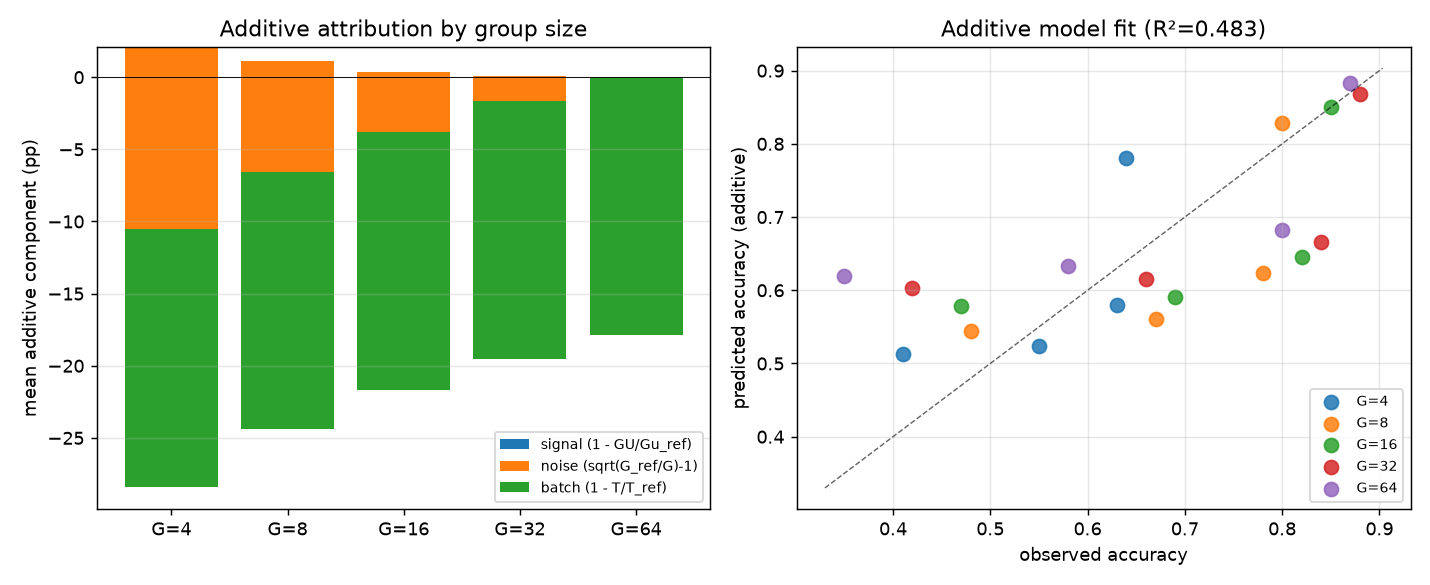
\includegraphics[width=0.95\linewidth]{figures/group_size_iter71_decomp.pdf}
  \caption{Additive decomposition of accuracy into signal,
           noise, and batch components.  \emph{Left:} mean additive
           component per group size, averaged across the four
           observed budgets.  \emph{Right:} predicted vs.\ observed
           accuracy; the additive model has $R^2 = 0.483$ on the
           20-row grid.  Each colour is one $G$; the dashed line is
           $y = x$.}
  \label{fig:group-size-iter71-decomp}
\end{figure}

\begin{figure}[ht]
  \centering
  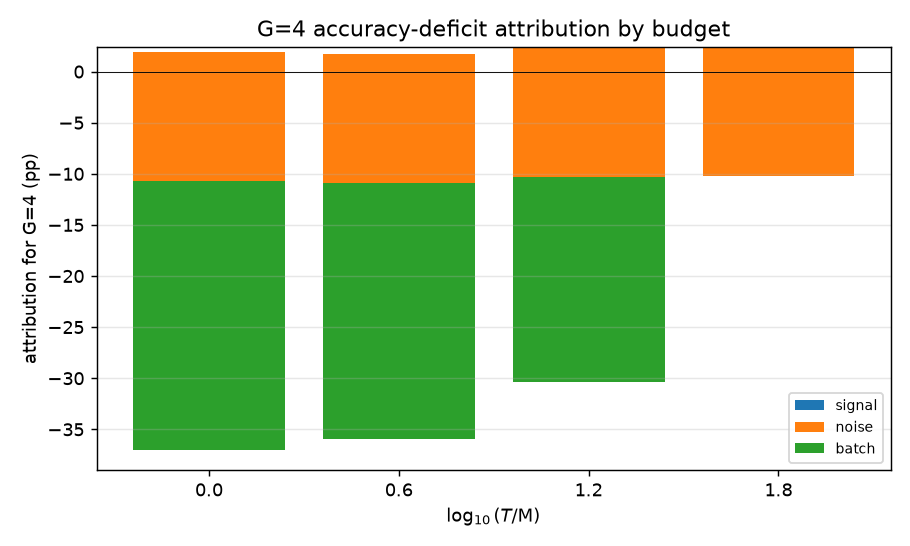
\includegraphics[width=0.85\linewidth]{figures/group_size_iter71_g4_budget.pdf}
  \caption{Attribution of the $G{=}4$ accuracy deficit across
           budgets $T \in \{1, 4, 16, 64\}\,\mathrm{M}$.  At small
           $T$ the dominant loss is the batch term (every $G$ pays
           it); at $T{=}64\,\mathrm{M}$ the dominant loss is the
           noise term $\sqrt{G_{\mathrm{ref}}/G} - 1$.}
  \label{fig:group-size-iter71-g4-budget}
\end{figure}